\documentclass[./00PhotoBox.tex]{subfiles}
\graphicspath{{\subfix{./img/}}}
\begin{document}

\chapter{Software-Entwicklung}
Für die Steuerung der Kameras und die anschließende Berechnung des 3D-Modelles muss ein Betriebssystem für das Kamerasystem und eine entsprechende Schnittstelle zu einer \gls{SfM}-Software geschaffen werden. Diese Entwicklung erfolgte hauptsächlich in Python in Form von Prototyping. Das Kapitel beschreibt die Anforderungen an die Software in \autoref{sec:Anforderungsanalyse}. Anschließend werden hieraus die Anwendungsfälle (\autoref{sec:Anwendungsfallmodellierung}) erarbeitet und abschließend die Implementation (\autoref{sec:Implementierung}) beschrieben.

\section{Anforderungsanalyse}
\label{sec:Anforderungsanalyse}

\subsection{Funktionale Anforderungen}
\begin{itemize}
    \item Die Kameras sollen zeitgleich auslösbar sein. Die Auslösung soll möglichst ver\-zögerungs\-frei erfolgen.
    \item Die Steuerung soll auch unabhängig von anderen Geräten möglich sein, beispielsweise per Tastensteuerung.
    \item Der Status des Systemes soll für den Nutzer erkennbar sein - auch ohne Anschluss eines Computers etc..
    \item Es sollen Passpunkte automatisch gefunden und und für die Bestimmung der äußeren Orientierung genutzt werden.
    \item Die Bilder sollen scharf und fokussiert sein.
\end{itemize}

\subsection{Schnittstellen}
\begin{itemize}
    \item Die Daten sollen intern gespeichert werden.
    \item Eine Speicherung auf tragbaren Speichermedien wie USB-Sticks soll möglich sein.
    \item Eine direkte Übertragung an \gls{SfM}-Software soll möglich sein.
\end{itemize}

\subsection{Nicht-funktionale Anforderungen}
\begin{itemize}
    \item Die Erfassung soll ohne weitere Hardware möglich sein. Das System soll unabhängig von Netzwerkanschlüssen etc. sein.
    \item Alle Kommunikation soll über WLAN erfolgen.
\end{itemize}

\section{Anwendungsfallmodellierung}
\label{sec:Anwendungsfallmodellierung}

Entsprechend der benötigten Schritte aus \autoref{c:photogrammmetrie} und \autoref{img:ablauf} wurde die Anwendungsfälle, die die Benutzeroberfläche ermöglichen soll, im Anwendungsfall-Dia\-gramm in \autoref{img:anwendungsfall} zusammengetragen.

\begin{figure}
    \centering
    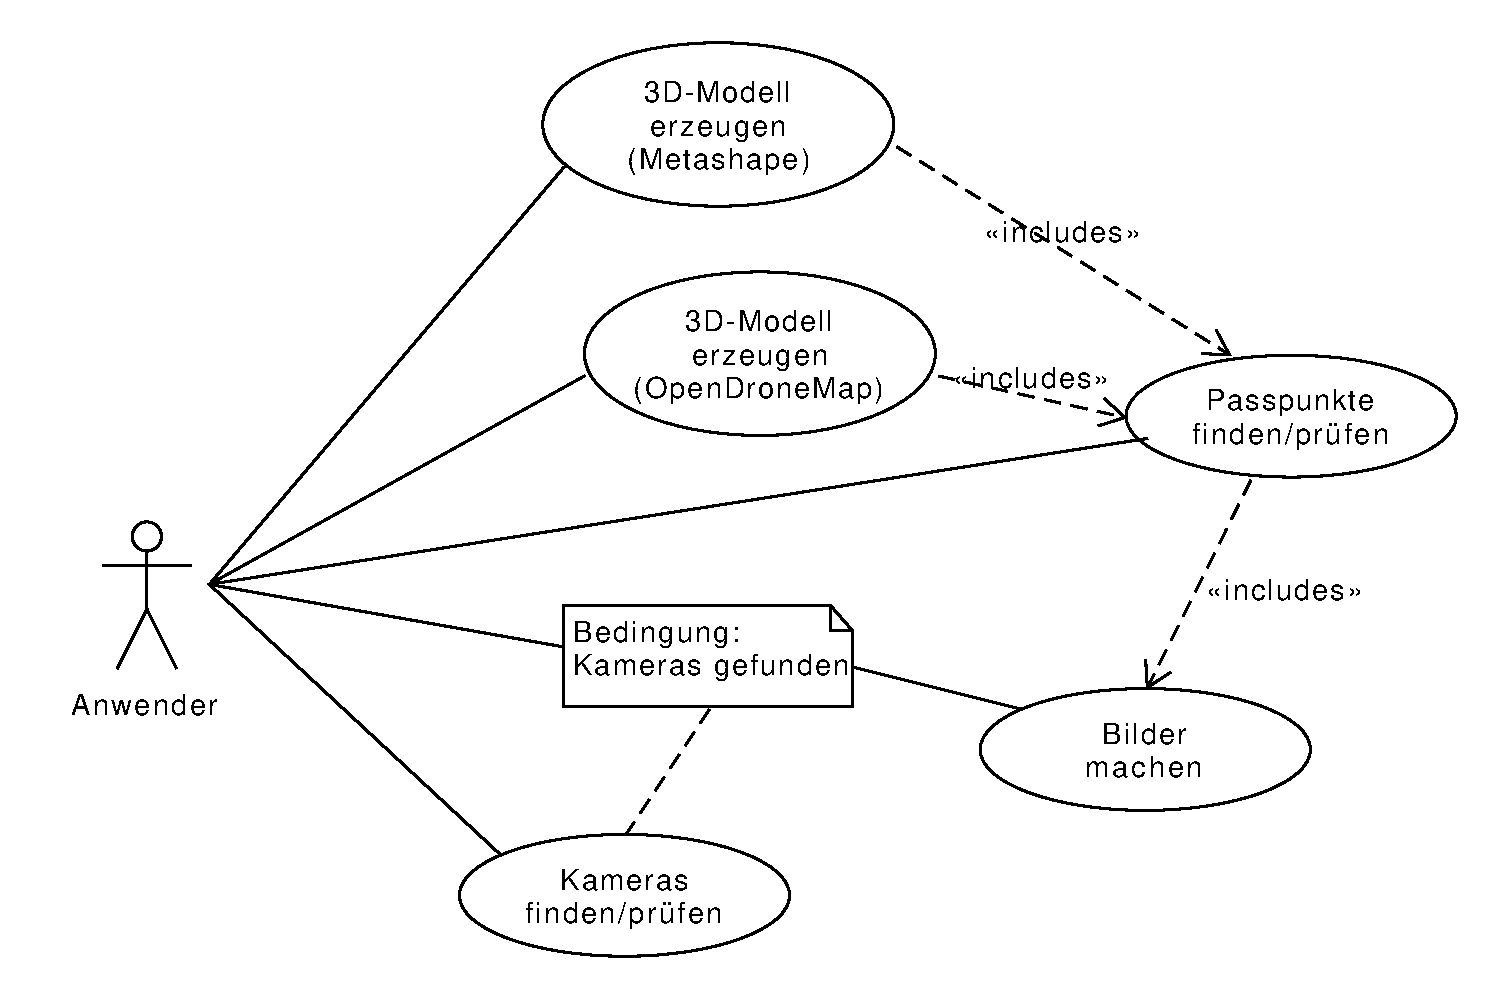
\includegraphics[width=1\textwidth]{./img/uml/uml_usecases.pdf}
    \centering
    \caption{Anwendungsfall-Diagramm} %Bildunterschrift
    \label{img:anwendungsfall} %ID fürs Bild
\end{figure}

Aus den benötigten Daten wurde das Domänen-Klassendiagramm aus \autoref{img:dokladia} erzeugt. Dieses zeigt vor allem die Abhängigkeiten der einzelnen Datensätze untereinander.

\begin{figure}
    \centering
    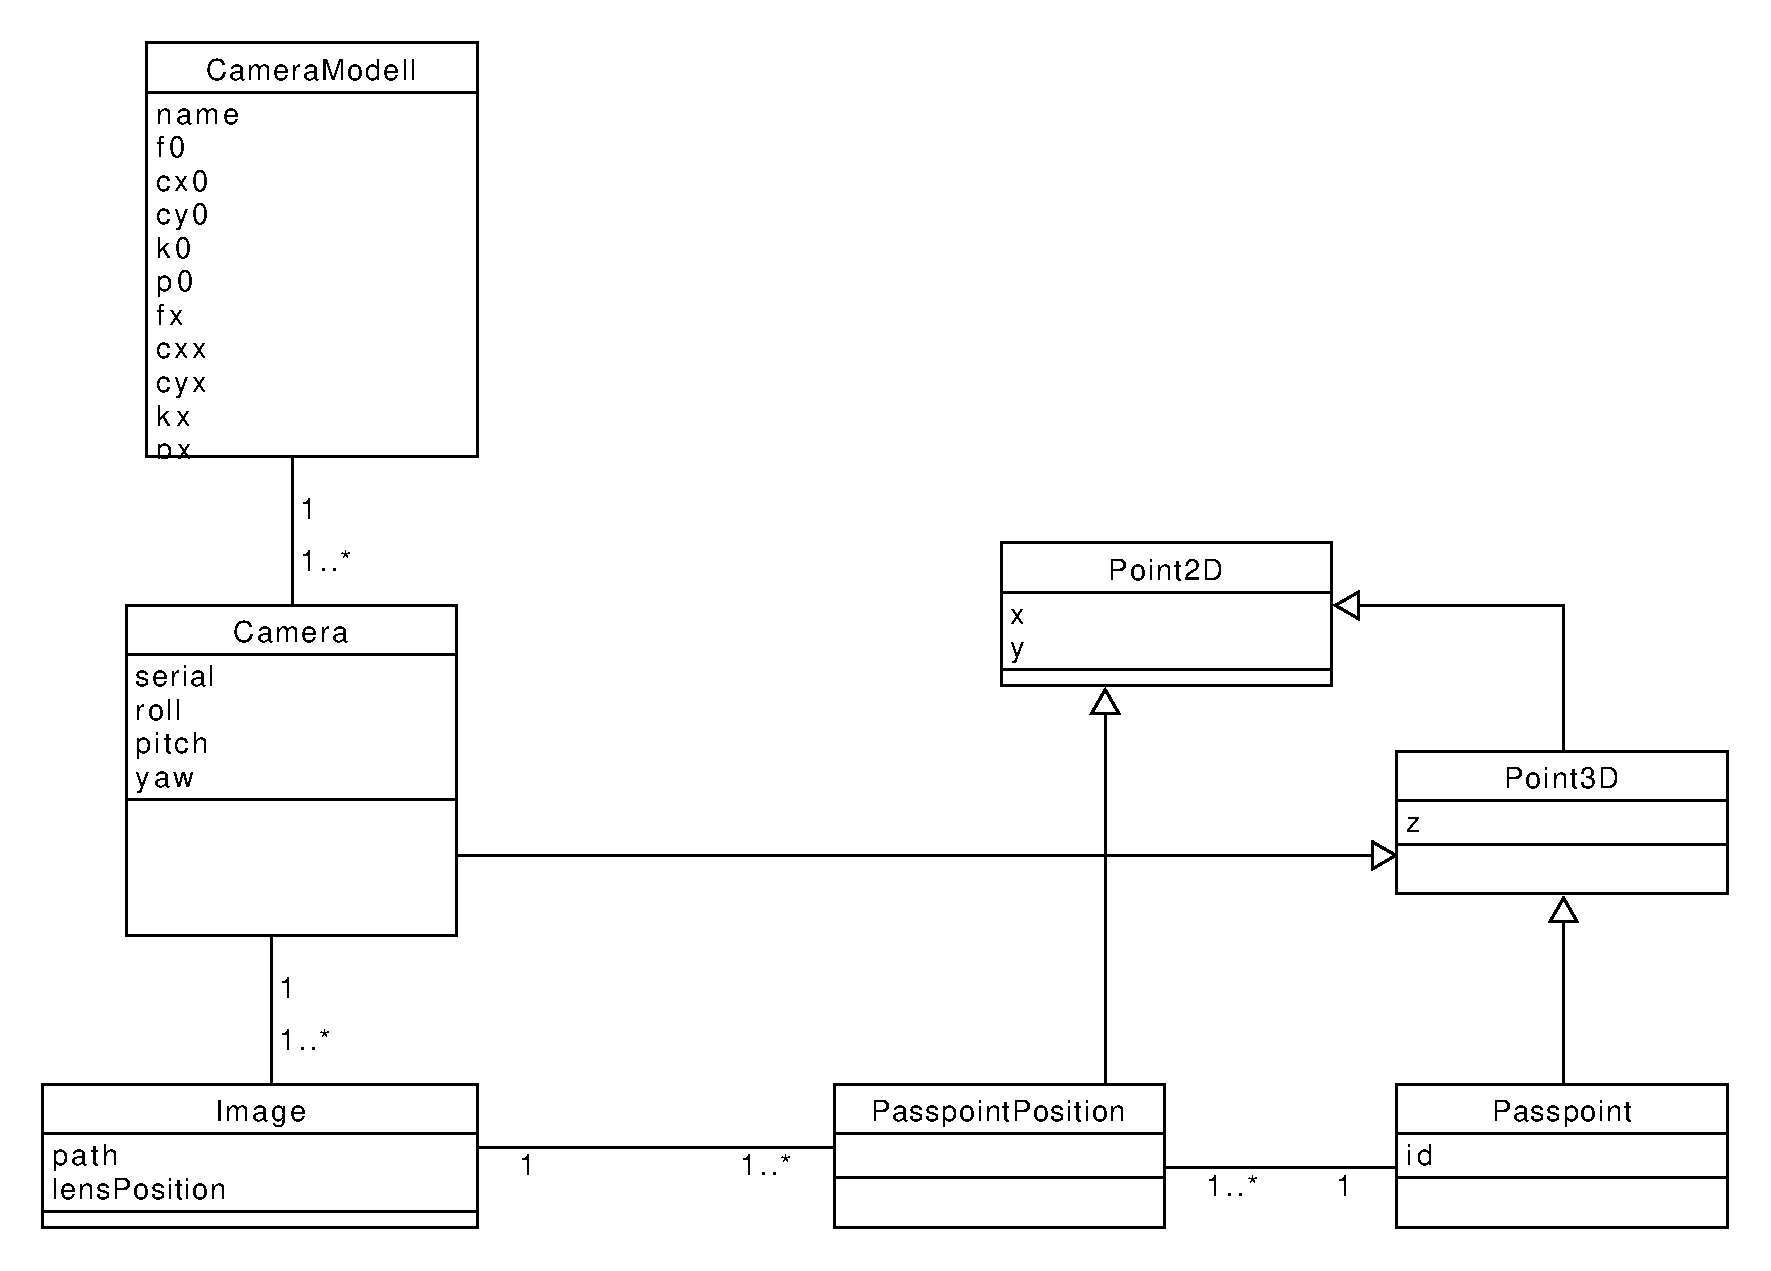
\includegraphics[width=1\textwidth]{./img/uml/uml_domain.pdf}
    \centering
    \caption{Domänen-Klassendiagramm} %Bildunterschrift
    \label{img:dokladia} %ID fürs Bild
\end{figure}

\section{Implementierung}
\label{sec:Implementierung}


Die Programmierung des Systemes erfolgte iterativ. Einzelne Arbeitspakete wurden in einem Jupyter-Notebook ausprobiert und dann, wenn dieser Schritt erfolgreich war, in den Gesamtworkflow integriert. Größtenteils wurden der Python-Code objektorientiert und typisiert geschrieben.



\subsection{Module auf den Raspberry Pi's (Python)}

\subsection{Allgemeine Module und Bibliotheken}
Es wurde, wenn möglich, auf fertige Python-Bibliotheken zurückgegriffen. Hierdurch sollte der Programmieraufwand verringert und auf bereits getesteten Code gesetzt werden. Die wichtigsten Bibliotheken sind:

\paragraph{OpenCV}
ist eine Bibliothek für Bildbearbeitung und maschinelles Sehen. Sie ist weit verbreitet und bietet viele photogrammetrische Funktionen. Hiermit wurde beispielsweise die Detektion von Markern durchgeführt und die Näherungswerte der Kameras berechnet.

\paragraph{NumPy}
bietet neben vielen weiteren Funktionen die Möglichkeit der Matrizenrechnung. Diese wurde für viele Berechnungen benötigt, beispielsweise für die Berechnungen der Kamera-Projektionen.

\paragraph{SciPy}
wurde für die Berechnung der Bündelblockausgleichung verwendet. Der manuelle Ansatz mit den Formeln aus \cite{luhmann} unter Nutzung von NumPy war sehr ressourcenlastig. Unter Verwendung von SciPy und der Projektionsgleichung konnte die Berechnungsdauer stark dezimiert werden.

\paragraph{Flask}
wurde genutzt um die Weboberfläche und die Datendownloads bereitzustellen. Hiermit wurde ein Webserver aufgesetzt, der die Daten der Kameras anzeigt und die Steuerung ermöglicht.

Außerdem wurden einige allgemeine Klassen erstellt, die in allen Modulen genutzt wurden. Diese sind in \autoref{img:uml_common} dargestellt. Diese steuern allgemeine Funktionen wie das Logging und das Auslesen der Konfiguration. Außerdem legen die Interfaces die Struktur der Datenübertragung zwischen den Raspberry Pi's fest.

\begin{figure}
    \centering
    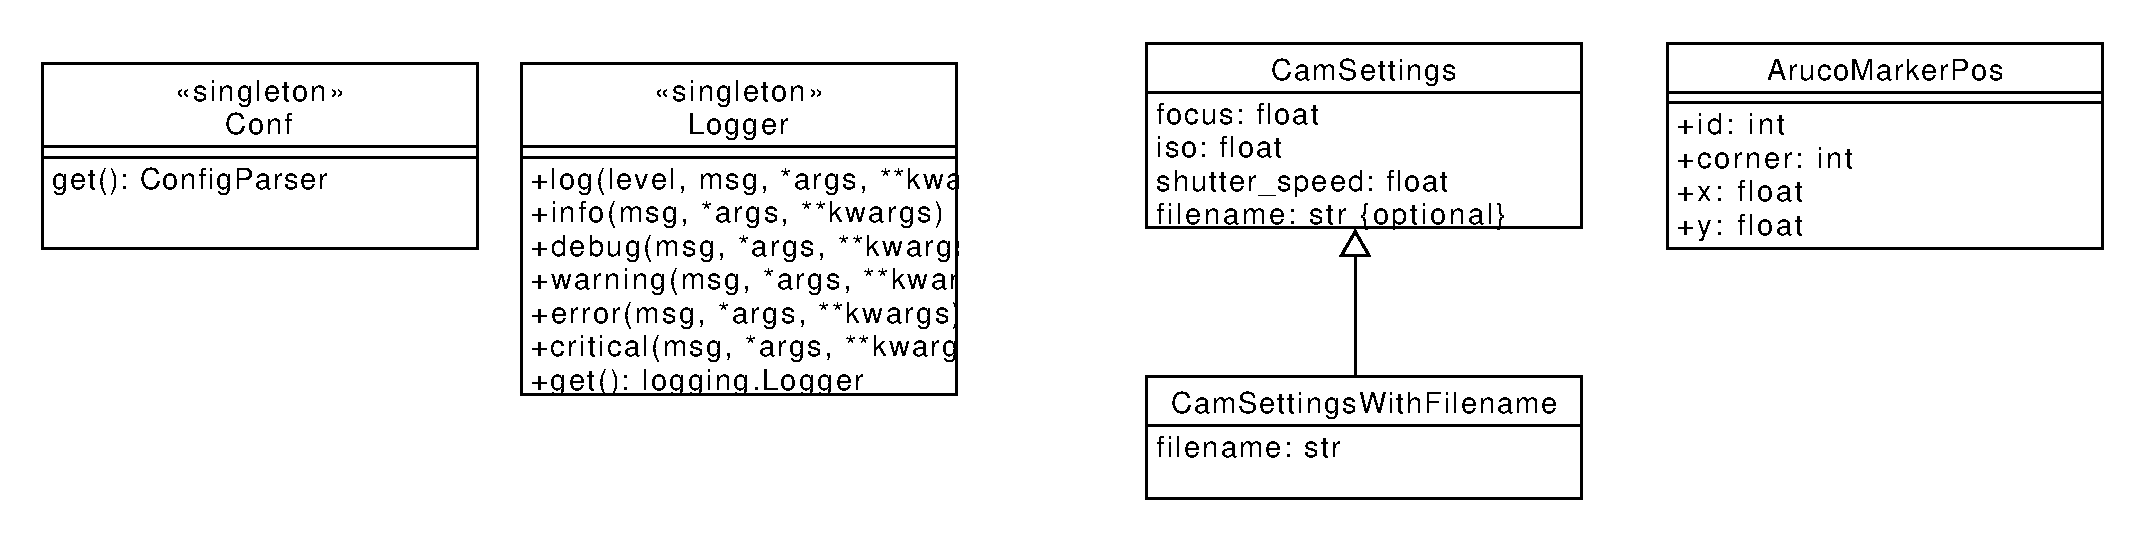
\includegraphics[width=1\textwidth]{./img/uml/uml_common_classdiagramm.pdf}
    \centering
    \caption{Common} %Bildunterschrift
    \label{img:uml_common} %ID fürs Bild
\end{figure}

\subsubsection{Kamera-Steuerung}
Die Raspberry Pi Zero W übernehmen die Steuerung der Kameras. Hierfür wurde ein Modul entwickelt, das die Kameras steuert, die Bilder aufnimmt und anschließend zur Verfügung stellt. Die Klassen sind in \autoref{img:uml_camera} dargestellt.

\begin{figure}
    \centering
    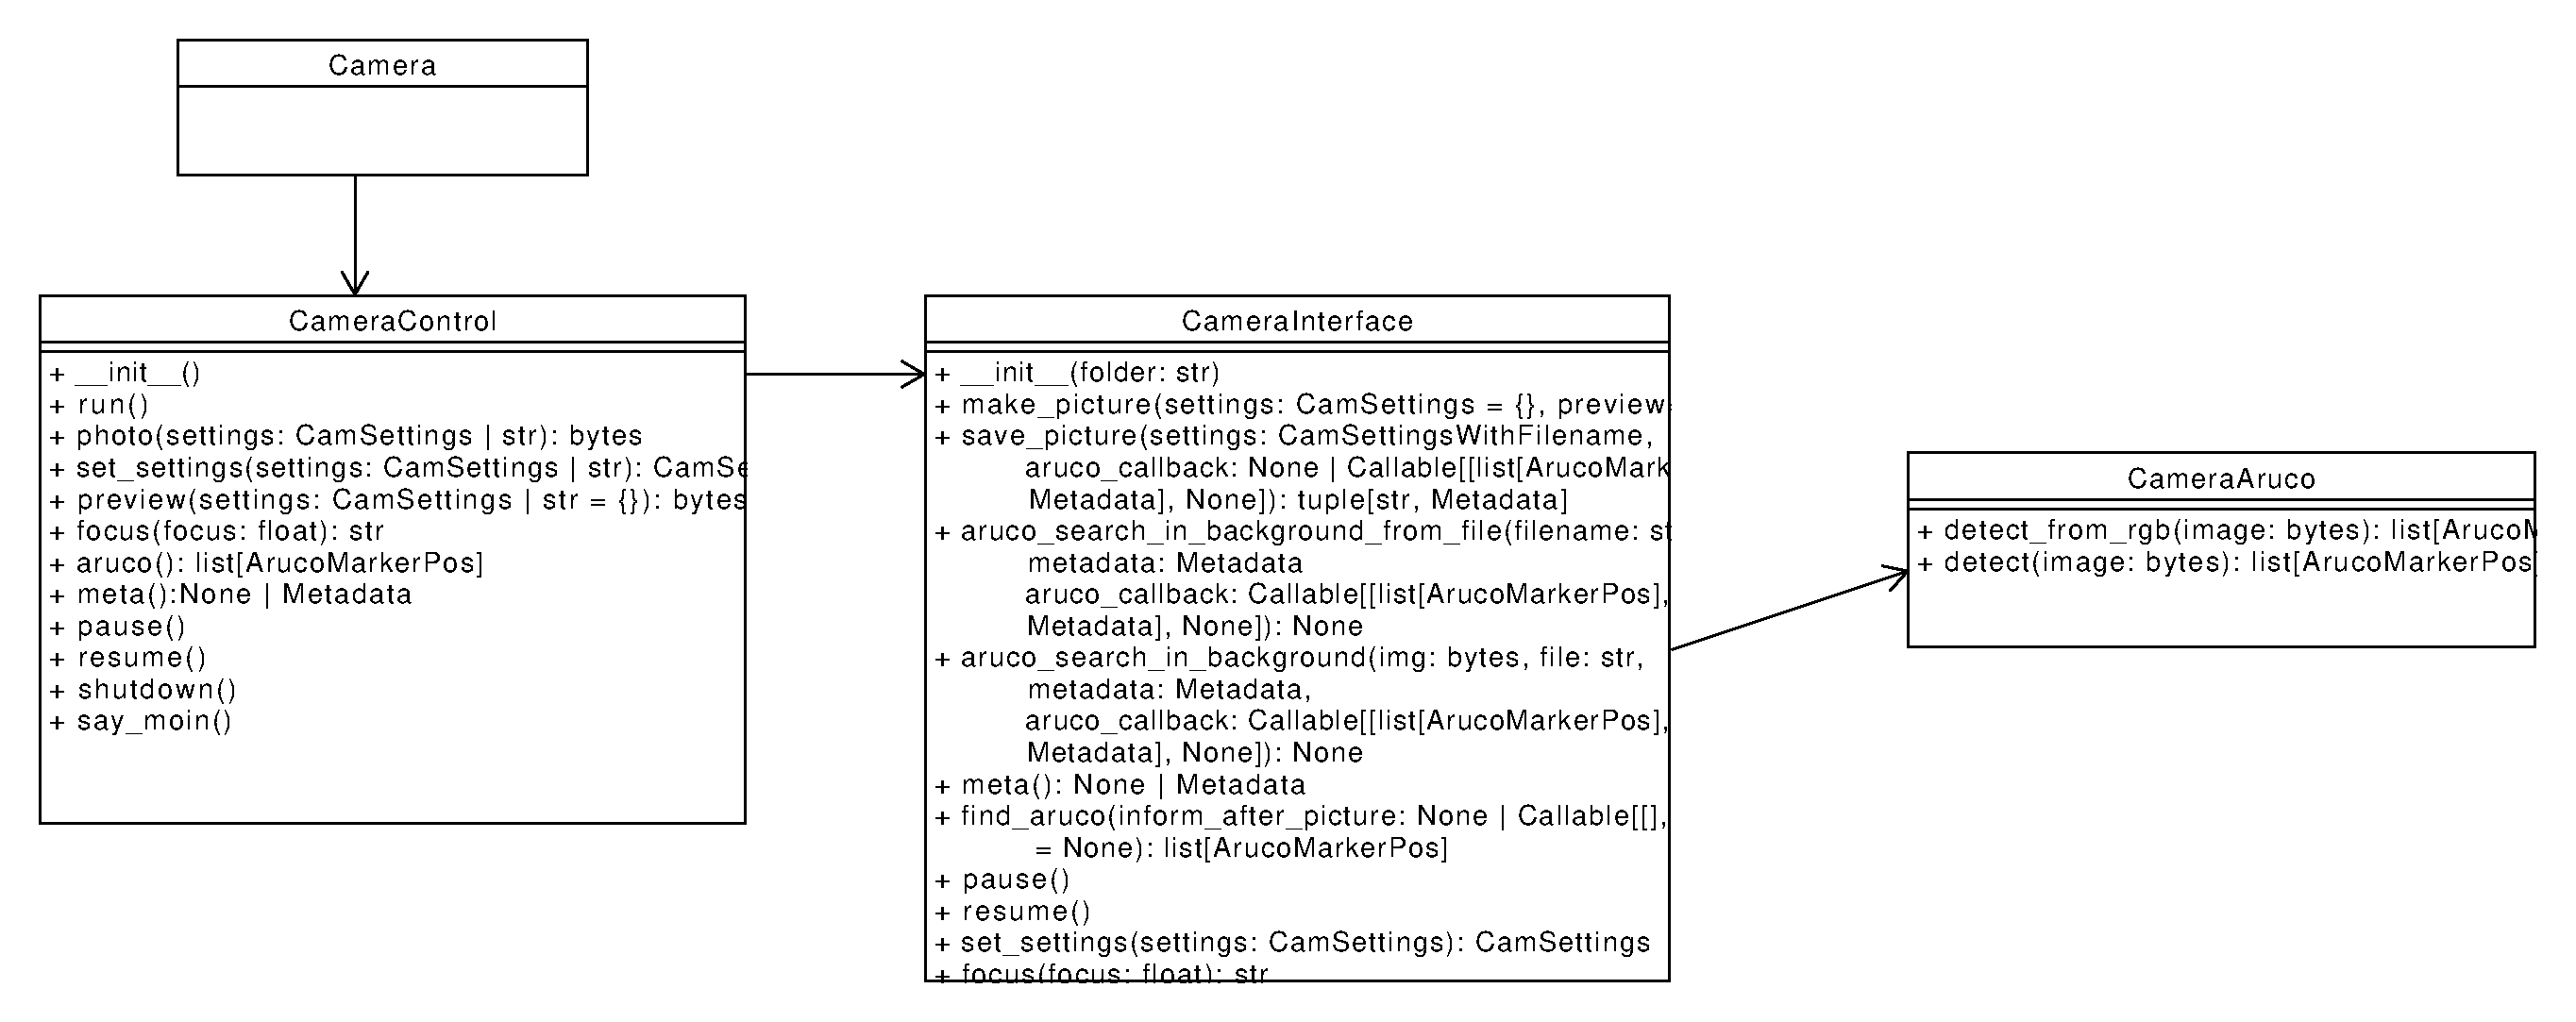
\includegraphics[width=1\textwidth]{./img/uml/uml_camera_classdiagramm.pdf}
    \centering
    \caption{Camera} %Bildunterschrift
    \label{img:uml_camera} %ID fürs Bild
\end{figure}

\subsubsection{Master-Steuerung}
\begin{figure}
    \centering
    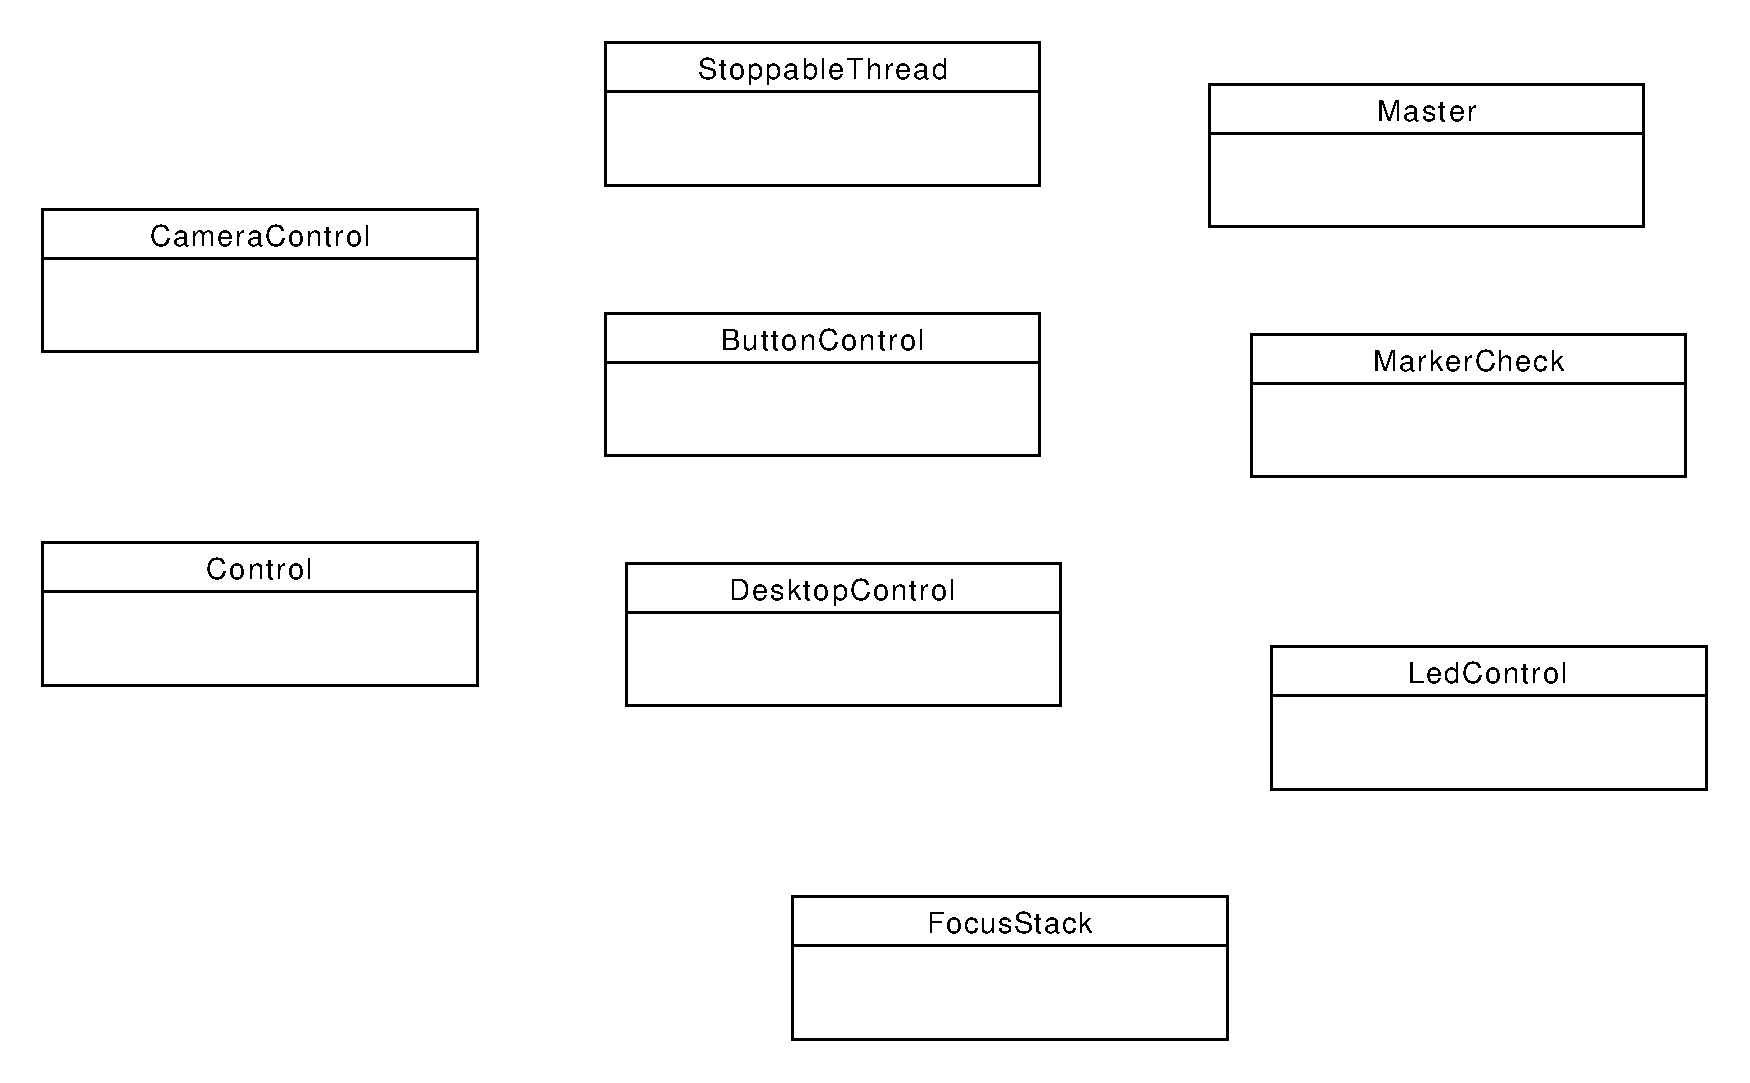
\includegraphics[width=1\textwidth]{./img/uml/uml_master_classdiagramm.pdf}
    \centering
    \caption{Master} %Bildunterschrift
    \label{img:master} %ID fürs Bild
\end{figure}

\subsubsection{Desktop-Programm (Java)}

\begin{figure}
    \centering
    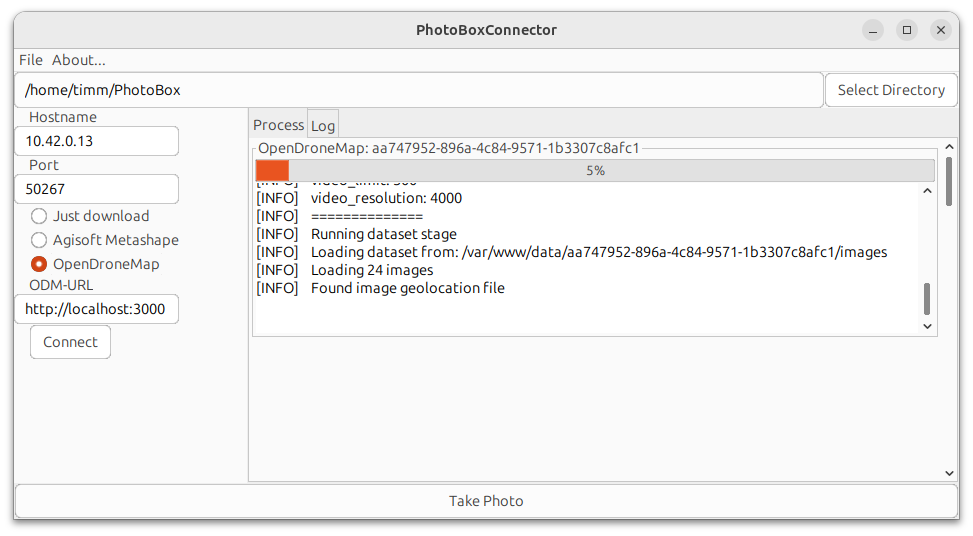
\includegraphics[width=1\textwidth]{./img/connector_screenshot.png}
    \centering
    \caption{Screenshot der Connector-Software unter Ubuntu 24.04} %Bildunterschrift
    \label{img:screenshot_connector} %ID fürs Bild
\end{figure}

\begin{figure}
    \centering
    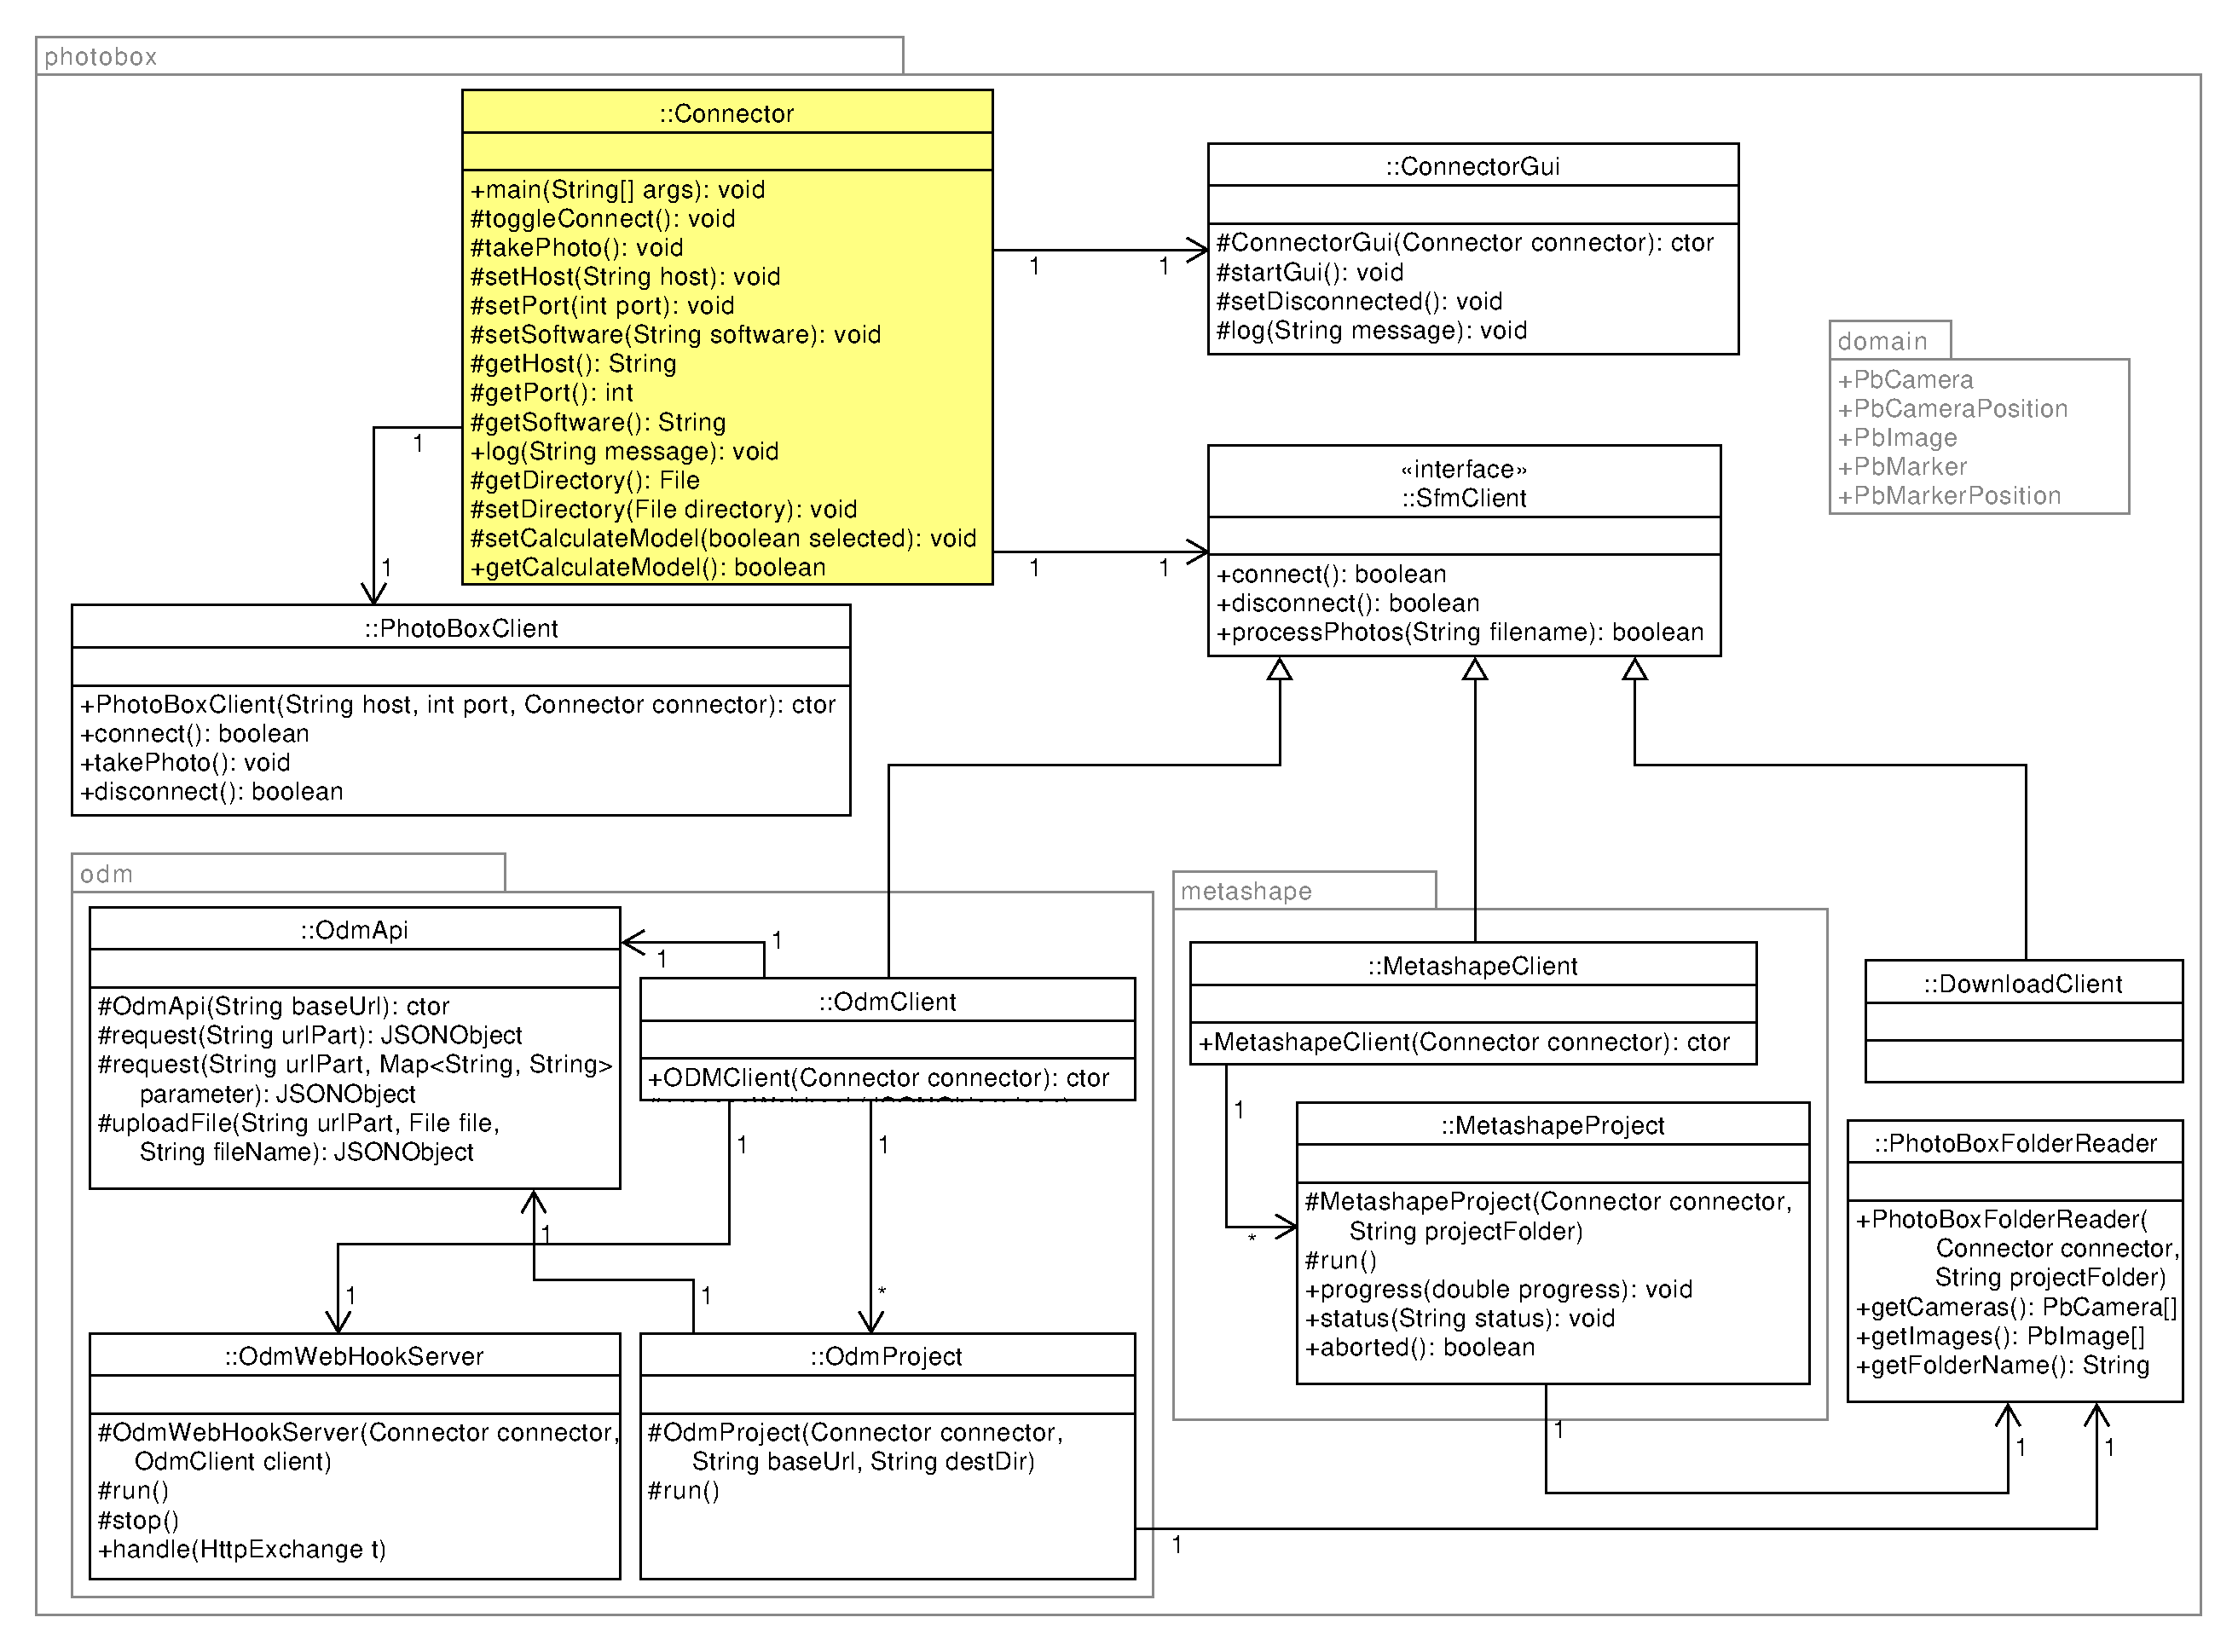
\includegraphics[width=1\textwidth]{./img/uml/uml_connector_classdiagramm.pdf}
    \centering
    \caption{Connector} %Bildunterschrift
    \label{img:uml_connector} %ID fürs Bild
\end{figure}

\biblio
\end{document}